\documentclass[onecolumn, draftclsnofoot,10pt, compsoc]{IEEEtran}
\usepackage{graphicx}
\usepackage{url}
\usepackage{setspace}
\usepackage{indentfirst}
\usepackage{geometry}
\usepackage[font=footnotesize]{caption}
\geometry{letterpaper, margin=0.75in}

% 1. Fill in these details
\def \CapstoneTeamName{			Code Monkeys in Space}
\def \CapstoneTeamNumber{		33}
\def \GroupMemberOne{			Mark Bereza}
\def \GroupMemberTwo{			Joseph Struph}
\def \GroupMemberThree{			Kevin Turkington}
\def \CapstoneProjectName{		NASA University Student Launch Initiative}
\def \CapstoneSponsorCompany{	Mechanical Engineering, OSU}
\def \CapstoneSponsorPerson{	Dr. Nancy Squires}

% 2. Uncomment the appropriate line below so that the document type works
\def \DocType{	%Problem Statement
				%Requirements Document
				Technology Review
				%Design Document
				%Progress Report
			 }
			
\newcommand{\NameSigPair}[1]{\par
\makebox[2.75in][r]{#1} \hfil 	\makebox[3.25in]{\makebox[2.25in]{\hrulefill} \hfill		\makebox[.75in]{\hrulefill}}
\par\vspace{-12pt} \textit{\tiny\noindent
\makebox[2.75in]{} \hfil		\makebox[3.25in]{\makebox[2.25in][r]{Signature} \hfill	\makebox[.75in][r]{Date}}}}
% 3. If the document is not to be signed, uncomment the RENEWcommand below
\renewcommand{\NameSigPair}[1]{#1}

%%%%%%%%%%%%%%%%%%%%%%%%%%%%%%%%%%%%%%%
\begin{document}
\begin{titlepage}
    \pagenumbering{gobble}
    \begin{singlespace}
        \hfill 
        \par\vspace{.2in}
        \centering
        \scshape{
            \huge CS Capstone \DocType \par
            {\large\today}\par
            \vspace{.5in}
            \textbf{\Huge\CapstoneProjectName}\par
            \vfill
            {\large Prepared for}\par
            \Huge \CapstoneSponsorCompany\par
            \vspace{5pt}
            {\Large\NameSigPair{\CapstoneSponsorPerson}\par}
            {\large Prepared by }\par
            Group\CapstoneTeamNumber\par
            \CapstoneTeamName\par 
            \vspace{5pt}
            {\Large
                \NameSigPair{\GroupMemberOne}\par
            }
            \vspace{20pt}
        }
        \begin{abstract}
        	The USLI project requires the creation of three distinct software products for its ultimate success: the team website, the rover autonomous movement software, and the avionics data logger software. Although all three members of Code Monkeys in Space will work on all three of these software products, each member has been assigned one of these products and will be ultimately responsible for its creation. The author of this paper is responsible for the rover autonomous movement software, and thus will explore the different options for operating system, software framework, and programming language used in its implementation.
        \end{abstract}     
    \end{singlespace}
\end{titlepage}
\newpage
\pagenumbering{arabic}
\tableofcontents
\clearpage
\section{Overview}
The ultimate goal of this project is a successful launch during the USLI event in April. A key part of a successful launch involves the deployment of the rover, its autonomous movement ending at least five feet from any part of the rocket body, and its deployment of solar panel cells. Since the rover's movement and solar panel deployment must be done autonomously, software must be created to instruct the rover how to accomplish these tasks. Although constructing software to simply tell the motor drivers to move the rover forward would be fairly trivial, such software would be inadequate for the purposes of this project. This is because the rover must be smart enough, for lack of a better term, to identify both the location of the rocket frame (in order to move away from it) and the location of insurmountable obstacles (so as to not get stuck). 

In order to provide the rover with adequate information and intelligence to accomplish its tasks, the mechanical and electrical engineering students on the team have decided to equip the rover with a Raspberry Pi 3 microcontroller, bidirectional motors and motor driver, two sonar sensors, an inertial measurement unit (IMU), and a GPS sensor. The software running on the microcontroller must then use data obtained from the motor driver and its various sensors to determine its distance from the rocket body, a viable path away from said body, and the state of the rover itself. The aforementioned state refers to whether the rover is successfully moving or whether it is stuck. This part is important because it is vital that the rover employs a different movement strategy in the event that the path finding algorithm fails and the rover finds itself stuck. 

The apparent complexity of obstacle avoidance, path finding, and computation of distance from a specific object motivated Code Monkeys in Space to use a software framework to assist in the creation of the rover software. Furthermore, additional points may be acquired during the competition for going 'above and beyond' the basic launch requirements. Utilizing robotics middleware would allow the team to more easily adapt the core rover software to do additional, potentially complicated, tasks if it is discovered that there is adequate time and resources to do so. Once it was decided that robotics middleware would be used, it became clear that the microcontroller must also run an operating system to facilitate its use. In light of this context, the questions this technology review will attempt to answer are the following:
\begin{enumerate}
\item What middleware or software framework should be used?
\item What operating system should the microcontroller run?
\item What programming language should be used to write the software?
\end{enumerate}
\section{Software Framework}
As mentioned previously, some form of robotics middleware will be used on the rover to avoid the problem of reinventing the wheel when it comes to complex robotics problems like path finding, object mapping, and sensor communication. Since none of the members of Code Monkeys in Space have experience with robotics middleware, the three selected for consideration were the three most popular robotics solutions that had libraries for the aforementioned tasks. These ended up being Mobile Robot Programming Toolkit (MRPT), Microsoft Robotics Development Studio (MRDS), and Robot Operating System (ROS).

MRPT is a software framework specifically designed to assist in the implementation of algorithms relating to Simultaneous Localization and Mapping (SLAM), computer vision, and obstacle avoidance \cite{MRPT}. Based on this description, this framework seems to be a good fit for the rover. The primary advantages of using MRPT compared to other middleware are that it is open source, it supports every major operating system (Windows, Linux, Mac OS X), and its fairly lightweight compared to other robotics middleware \cite{MRPT}. One large downside to MRPT, however, is that all of its libraries are in C++, meaning it has no support for other programming languages. Additionally, MRPT is fairly low on the software stack, meaning it cannot nest other frameworks within itself like ROS. Finally, MRPT is a smaller project compared to ROS and MRDS, lacking the sheer number of contributors and update frequency of ROS and the vast corporate resources of MRDS.

According to its MSDN page, Microsoft Robotics Developer Studio "is a Windows-based environment for hobbyist, academic and commercial developers to create robotics applications for a variety of hardware platforms" \cite{MRDS}. One advantage to using MRDS over ROS or MRPT is that MRDS is based on and integrates with Visual Studio, a powerful and widely-used IDE. Additionally, MRDS supports both C\# and its own visual programming language as means of creating software. Microsoft additionally advertises the framework's support for handling asynchronous input from multiple sensors and 3D simulation, but these functionalities can also be achieved with the other two frameworks under consideration. The primary disadvantage of using MRDS is its shoddy support with regards to both Raspberry Pi hardware and operating systems. Although it is possible, with some hacking, to run MRDS on any Windows-based operating system, MRDS is officially only supported on Windows 7, which cannot run on the Raspberry Pi. Furthermore, selecting this middleware would force the team to use Windows 10 IoT (because it is the only Windows-based OS that will run on the Raspberry Pi) and C\# (being its only supported conventional programming language). Finally, it is important to note that MRDS is no longer maintained by Microsoft and the last update to it was made in 2012. Because the software is closed source, it is unlikely that it will ever be updated again, unlike ROS and MRPT, which are updated regularly.

According to its website, The Robot Operating System (ROS) is "a collection of tools, libraries, and conventions that aim to simplify the task of creating complex and robust robot behavior across a wide variety of robotic platforms" \cite{ROS}. ROS is the most popular robotics software framework, has the most contributors of the open source options, and has the largest number of existing libraries. Additionally, ROS has significantly better language options than its competitors, having complete implementations in Python, C++, and Lisp and partial implementations in Java and Lua \cite{ROS2}. Moreover, several mechanical and electrical engineering students on the team have experience with ROS, making it easier to communicate work done in software to non-software team members. Finally, ROS can integrate with other software frameworks like Orocos and Player and even has existing wrappers for MRPT packages. The downsides to ROS are that it does not support Windows and it has a fairly steep learning curve. These downsides are fairly minor when one considers that the microcontroller will almost certainly be running some form of Linux and that Code Monkeys in Space will have plenty of time to become familiar with whatever framework is selected while the team as a whole waits for parts to arrive and the first rover prototype to be built. Since it is apparent that the advantages of using ROS far outweigh its disadvantages, it will be used to aid in developing the rover software.

\section{Operating System}
Selecting the best operating system to run on the Raspberry Pi 3 microcontroller is only important in that it should not impair the rover's ability to perform its required tasks and that it supports the desired robotics middleware. The three operating system options considered were Ubuntu, Windows 10 IoT Core, and Raspbian. These three were considered because they are officially supported by the Raspberry Pi \cite{RaspberryPi}. Additionally, it was important to select at least one Linux OS and one Microsoft OS because ROS is only officially supported on Unix-like operating systems \cite{ROS_OS} and MRDS can only run on Windows operating systems \cite{MRDS_OS}.

Ubuntu for Raspberry Pi comes in two flavors: regular Ubuntu and Ubuntu Core. The benefits of using Ubuntu are that it is a relatively user-friendly distribution of Linux, ROS and MRPT support it, it is updated frequently, and there is a lot of support and documentation for it as a result of its popularity. The flexibility between the regular and core versions can also been seen as a positive trait. Ubuntu Core is different from standard Ubuntu in that it is stripped-down, uses a completely different package system, isolates application dependencies to allow for better environment control, and utilizes a read-only file system with two partitions to allow for rollbacks \cite{UbuntuCore}\cite{UbuntuCoreAnswer}. Both versions, however, have their problems. For starters, standard Ubuntu isn't very lightweight. Indeed, it is an operating system designed for desktop computers and features a full GUI desktop. This is an issue due to the limited memory and processing power of the Raspberry Pi. Ubuntu Core, while certainly more lightweight, is also not a great candidate for several reasons. For one, its immutable file system may prove to be an obstacle when developing software for the rover. Additionally, little is gained from the overhead involved with isolating application dependencies or maintaining a second partition for rollbacks under the context of this project. Finally, there are very few applications available via the Snappy packages it uses due to how young the operating system is, meaning less options when it comes to installing applications not from source. 

Windows 10 IoT Core is another option. It is essentially a lightweight version of the Windows 10 operating system designed to run on small systems like IoT devices, as the name would imply. One  advantage of Windows 10 IoT Core is that it has a fairly shallow learning curve due to it being very similar to the user-friendly and ubiquitous desktop Windows. Additionally, it would allow for the use of some proprietary Microsoft software like Visual Studio directly on the Raspberry Pi. There are, however, numerous downsides to Windows 10 IoT Core. First off, ROS does not support it. Secondly, there is a very limited list of hardware supported by Windows 10 IoT Core \cite{WinHardware}, meaning that the specific sensors and other hardware selected for the rover might not even be recognized by the OS. Third, the operating system is neither free nor open source, unlike the other two operating systems under consideration. Finally, the supposed advantage of being able to run proprietary Microsoft software is not very useful when one considers that the Raspberry Pi will only be running the minimal software necessary to accomplish its tasks since the development and testing of the software can and should be done remotely.

Raspbian is a Debian-based Linux distribution and is the Raspberry Pi Foundation's official supported operating system \cite{Raspbian}. As the name would imply, it was specifically designed to run on the Raspberry Pi and is optimized for its hardware \cite{Raspbian2}. Being a Linux distribution, it is supported by both ROS and MRPT. These factors alone make it a strong contender for the operating system of choice for the microcontroller. Beyond that, Raspbian is more lightweight than standard Ubuntu (even headless) and is not burdened by the two-partition read-only filesystem of Ubuntu Core or its limited packages. Raspbian is also far superior to Windows 10 IoT Core for this project because it is Linux and thus is open-source, is free, and has extensive hardware support. In light of these considerations, Raspbian has been chosen as the operating system that will run on the rover's microcontroller.

\section{Programming Language}
The final point of consideration is what programming language the rover software should be written in. The languages to be considered are largely a function of what languages are supported by the software frameworks under consideration. Since MRPT only supports C++ and MRDS only supports C\#, they must be considered. Python is the third language under consideration because it is supported by ROS and is fairly flexible. Although what programming language is "correct" for a given software project can often be very subjective, there are some specific language qualities that are desirable for this project:
\begin{itemize}
\item Team Familiarity:\\Using a language that the CS team members are already
familiar with or least similar in syntax to one they are familiar with would
certainly help streamline the development process.
\item Memory Management:\\Using a language with built-in garbage collection
would help avoid a lot of runtime errors related to invalid memory access
and prevent memory leaks from occurring.
\item Multi-Processing:\\Since the microcontroller selected, a Raspberry Pi 3, uses
a multi-core CPU, using a language that can effectively leverage simultaneous use of
multiple cores would help the team make the most of the microcontroller's
capabilities.
\item Ease of Debugging:\\Given the perceived complexity of the rover's software,
the team anticipates a lengthy testing and debugging stage. Languages that
are easier to debug are obviously preferable.
\item Memory Overhead:\\In light of the limited memory available on the
Raspberry Pi, languages that make efficient use of memory are desirable.
\item Performance:\\Although this property is generally inversely-correlated with
automatic memory management, languages that can achieve the same
functionality in a smaller number of clock cycles are preferable.
\end{itemize}
\par Each of these desired features was then assigned a weight from 1 to 10 (1 being not important at all and 10 being critically important) based on their perceived relative importance. Then, each of the languages under consideration was given a subjective grade from 1 to 10 (1 being very poor and 10 being very good) for each category. The result of this approach can be seen in Figure 1.\\ \\
\begin{minipage}{\linewidth}
\begin{center}
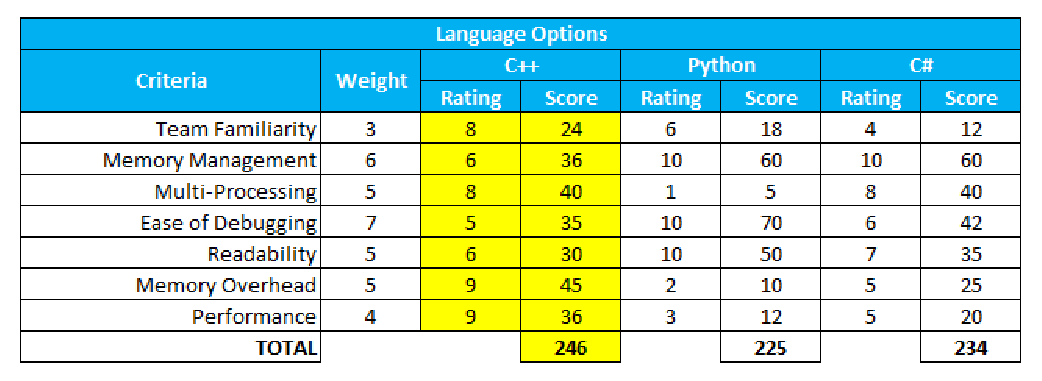
\includegraphics[width=\textwidth]{design_matrix.eps}
\captionof{figure}{Design matrix evaluating the viability of C++, Python, and C\# based on various criteria at various weights.}
\end{center}
\end{minipage}\\ \\
\par Based on this evaluation, C++ is the best option. It is a mature language with extensive standard libraries and the recent versions (C++11, C++14, and C++17) support most modern programming
language features like reflection, constant expressions, lambda expressions, type deduction, and threading. Additionally, C++ is more efficient than both Python and C\# in terms of CPU and memory usage. C++'s biggest weakness in this context is its lack of automatic memory management, but this has become less of an issue with the adoption of smart pointers into its standard. Python, although being easy to read, write, and debug, is ultimately a subpar choice because its Global Interpreter Lock (GIL) prevents it from fully leveraging the Raspberry Pi's quad-core CPU. While C\# does support multi-processing,
it loses to C++ in performance and would force the team to utilize the vastly inferior MRDS framework and Windows 10 IoT operating system since it is not supported by either ROS or MRPT. Consequently, C++ was selected as the language the rover software will be written in.
\section{Conclusion}
Although compatibility between framework and language and compatibility between framework and operating system were major considerations in these decisions, the decisions were made in parallel, not in series. In other words, although compatibility was a consideration, choices were not made under the assumption that another choice had already been made. This is the reason why C\# was still considered as a potential language option even though the selected software framework, ROS, does not support it. This was done in order to prevent granting excessive weight to the first decision and to prevent the final decision from simply 'falling out' as a result of compatibility constraints introduced by the first two decisions.

In conclusion, the rover will feature a Raspberry Pi 3 microcontroller running the Raspbian operating system because it is the operating system specifically designed to run on a Raspberry Pi. The rover software will utilize the Robot Operating System as a software framework because it is more powerful than the alternatives and provides the greatest flexibility with regards to programming languages. The software itself will be written primarily in C++ because it is efficient and capable of fully utilizing the Raspberry Pi's quad-core CPU. 
\clearpage
\bibliographystyle{IEEEtran}
\bibliography{mybib}
\end{document}